\chapter{Imbalance Detection Algorithm} % Chapter title
\label{ch_detection_algorithm}

%----------------------------------------------------------------------------------------
%	Overview
%----------------------------------------------------------------------------------------
\section{Overview}
A rotor imbalance can causes problems and failures with the turbine, so it is important to detect the ``state" of the turbine using some measured input.  Turbine dynamics are complicated, vary between different systems and can be dependent on many variables.  An effective way to develop a model that is optimized for each different turbine is to use machine learning (ML).  Machine learning is the study of algorithms that build mathematical models to perform specific tasks without explicit instructions.

\subsection{Machine learning background}
The 2 main types of machine learning algorithms are supervised and unsupervised learning.  Supervised algorithms assume that each data set is assigned an output, while unsupervised algorithms take a data set of only inputs and attempt to create groups and classes from the input data.  For this application, each measurement data set from the turbine will be manually labeled as ``good" or ``bad" (or as ``balanced"/``unbalanced"), which is a type of supervised learning.

Machine learning algorithms also fall into the ``regression" or ``classification" categories.  Regression algorithms are used if the output is a continuous function, while classification algorithms are used if the output falls into distinct classes.  The output for the turbine detection algorithm is the state of the turbine (balanced/imbalanced), which is a discrete classification.

Knowing that the ML algorithm must be a classification, supervised model, the specific algorithm choice can be narrowed down.  Some of the common algorithms are logistic regression (this can be used as a classification algorithm even though it is called ``regression"), k-nearest neighbor, and neural networks.  This paper will analyze each of these models and apply them to the experimental turbine data.

\section{The training data}
Typically, it is common for machine learning algorithms to split the data into test and training sub groups.  This allows the accuracy of the models to be trained and evaluated on different data sets.  The input data for the turbine is a 256-point frequency spectrum of the acceleration data at the top of the tower.  This data is obtained using the LifeLine system, which includes an accelerometer and a STM32 microprocessor.  This device is placed at the top of the tower and powered directly from the turbine.  Ideally, this device would significantly drop the clock rate of the processor or swap out the processor for an extremely low-power one.  This would allow the device to be wireless and have a reasonable operation time for each battery charge.  Figure \ref{fig:LL_spectrogram} shows a spectrogram of the measured acceleration data from the LifeLine device.  A spectrogram is a way to visualize frequency data over time in a 2-dimensional figure, where the magnitudes of each frequency component are represented by a different color.  The spectrogram shows that there is a strong frequency component at about 2.4 Hz (the rotor frequency) that is constant throughout most of the operation.

\begin{figure}
	\centering
	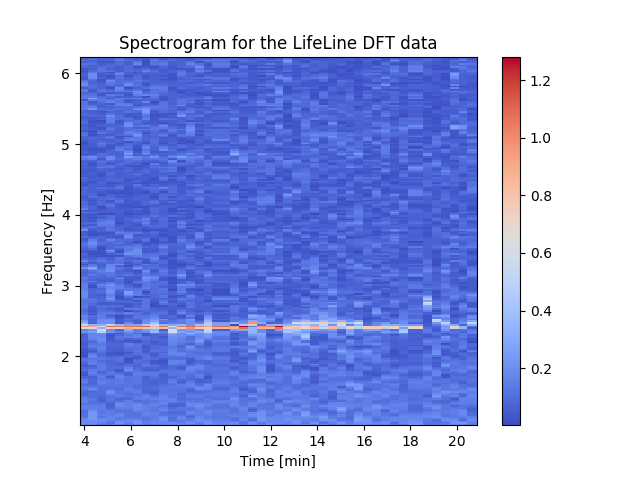
\includegraphics[scale=0.8]{LL_spectrogram}
	\decoRule
	\caption{This figure shows the spectrogram of the tower accelerations.}
	\label{fig:LL_spectrogram}
\end{figure}

Currently, only a single set of about 100 training examples exists.  The data can be separated into 2 classes; however, there is no information about which is the \textit{balanced} and \textit{imbalanced} classes.  To properly train the machine learning models, more data is required.  Despite the lack of available data, this paper will discuss the methods and implementations of each algorithm using the limited data set.


\section{K-Nearest Neighbor algorithm}
\section{About the algorithm}
The k-nearest neighbor (KNN) algorithm is one of the simplest models, but can be the most accurate and powerful when dealing with fairly small data sets.  This model essentially ``memorizes" the training data and plots the points in $n$-dimensional space.  The classification of a new point is calculated based on the distances between the new point and the training points.  For example, Figure \ref{fig:knn_visualization} shows a visualization of the classification process for a 2-class system.  Since this algorithm uses all of the training data in memory, it becomes very slow with many inputs, and many training data sets.  The example in Figure \ref{fig:knn_visualization} is a 2-dimensional problem (only 2 inputs) with only a few data points, so the KNN algorithm works very well.


\begin{figure}
	\centering
	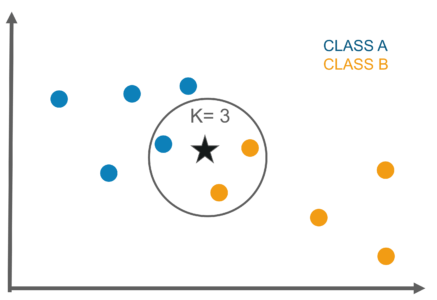
\includegraphics[scale=0.4]{knn_visualization}
	\decoRule
	\caption{A visualization of the KNN algorithm \cite{knn_python}.  The training data for a 2-class problem with 2 inputs is shown as blue and orange dots.  For $K=3$, a circle is drawn around the new point (star) until 3 training data points fall within the circle.  The classification of the new point is then determined by the majority of the points inside the circle.  In this case, there are more \textit{Class B} points than \textit{Class A} points, so the new point (star) will be classified as \textit{Class B}.}
	\label{fig:knn_visualization}
\end{figure}

The K-NN algorithm uses a "majority voting" method where the Euclidian distance between all the training data points and the test data is calculated.  This model assumes there is a relatively equal amount of balanced rotor experimental data and imbalanced experimental rotor data, which means the sample weighting can be uniform.  If there is a much higher frequency class (for example, much more balanced experimental data), this class will tend to dominate the calculations regardless of the actual class of the test data.

The number of neighbors, $k$, is chosen to be 5 for this algorithm (using trial and error).  A larger value of $k$ will reduce the classification noise, but the boundaries are much more general and not as tuned to the training data.  A lower value of $k$ will match the model very closely to the training data, but may add noise into the classification process.

The Euclidean distance is simply the distance between the data points.  This equation is shown below:

\begin{equation}
	d = \sqrt{\sum{\left(x_{i,a}-x_{j,a}\right)^2}}
\end{equation}

\subsection{Choosing the data}
The KNN algorithm works well on small data sets, so the DFT data should be pre-processed and cut down to a smaller, 2-dimensional data set.  Based on a simplified dynamic model of the turbine tower, a rotor imbalance will cause a high frequency excitation at the rotor frequency.  Using the maximum frequency component of the experimental DFT data and the corresponding frequency is a good way to capture enough information about the tower, while also reducing the data set from 256 input points to only 2 input points.

Figure \ref{fig:single_dft} shows the frequency spectrum from a single DFT calculation.  To convert this data into 2-dimensional data for the KNN algorithm, the peak value and corresponding frequency are extracted from this data.  For example, Figure \ref{fig:single_dft} would produce a 2-dimensional data set as shown in Equation \ref{eq:2d_data}.
\begin{equation} \label{eq:2d_data}
	[frequency, amplitude, class] = [2.3, 1.0, Class A]
\end{equation}

\begin{figure}
	\centering
	\includegraphics[scale=0.4]{single_dft}
	\decoRule
	\caption{This figure shows a single DFT result (a single column from Figure \ref{fig:LL_spectrogram}).}
	\label{fig:single_dft}
\end{figure}

By converting the entire data set for all training examples into 2-dimensional data, the data in Figure \ref{fig:LL_spectrogram} can be represented as the data in Figure \ref{fig:max_balanced_freq_mag}.

\begin{figure}
	\centering
	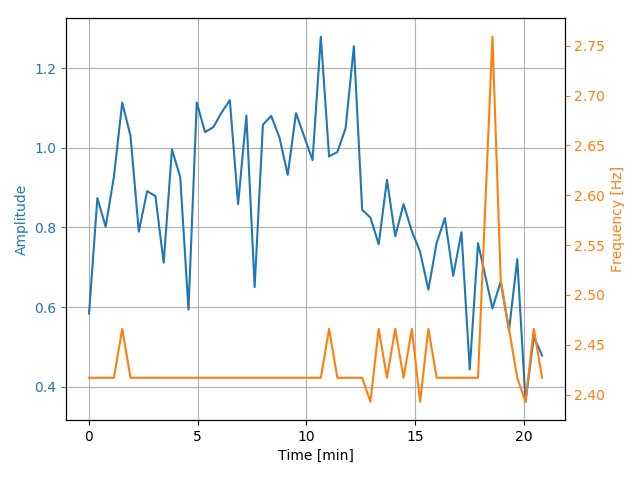
\includegraphics[scale=0.8]{max_balanced_freq_mag}
	\decoRule
	\caption{This figure shows a the 2-dimensional data used as an input to the KNN classification algorithm.}
	\label{fig:max_balanced_freq_mag}
\end{figure}


\subsection{Algorithm Results}
To apply the algorithm, the data is converted into short lists containing a maximum amplitude, a corresponding frequency value, and the known class (Equation \ref{eq:2d_data}). For this test, there are 55 experimental DFT results for \textit{Class A} and 55 experimental DFT results for \textit{Class B}. 

Training the KNN model is extremely fast and only involves storing all of the training data in memory.  When the algorithm is applied to new test examples, the results can be visualized in a confusion matrix \cite{confusion_matrix} as shown in Equation \ref{eq:knn_confusion_matrix}.  A confusion matrix is a common tool used to describe the performance of a classification algorithm.  This is an $n$ by $n$ matrix (where $n$ is the number of classes) that essentially shows the amount of correct and incorrect guesses for each class.  Table \ref{t:confusion_matrix_ex} shows a labeled version of the confusion matrix shown in Equation \ref{eq:knn_confusion_matrix}.

\begin{equation} \label{eq:knn_confusion_matrix}
C_{confusion} = 
\begin{bmatrix}
	12 & 1 \\
	3 & 6
\end{bmatrix}
\end{equation}

\begin{table}[]
\centering
\caption{An example of the terminology for the confusion matrix in Equation \ref{eq:knn_confusion_matrix}. \textit{Class A} and \textit{Class B} represent the different classes of data.  These can be related to a \textit{balanced} and \textit{imbalanced} rotor with proper data set labels.}
\label{t:confusion_matrix_ex}
\vspace*{0.2in}
\begin{tabular}{lllll}
\cline{2-3}
\multicolumn{1}{l|}{}                      & \multicolumn{1}{l|}{\textbf{Predicted Class A}} & \multicolumn{1}{l|}{\textbf{Predicted Class B}} &  &  \\ \cline{1-3}
\multicolumn{1}{|l|}{\textbf{Actual Class A}}  & \multicolumn{1}{l|}{12}                     & \multicolumn{1}{l|}{1}                       &  &  \\ \cline{1-3}
\multicolumn{1}{|l|}{\textbf{Actual Class B}} & \multicolumn{1}{l|}{3}                      & \multicolumn{1}{l|}{6}                       &  &  \\ \cline{1-3}
                                           &                                             &                                              &  & 
\end{tabular}
\end{table}


\begin{figure}
	\centering
	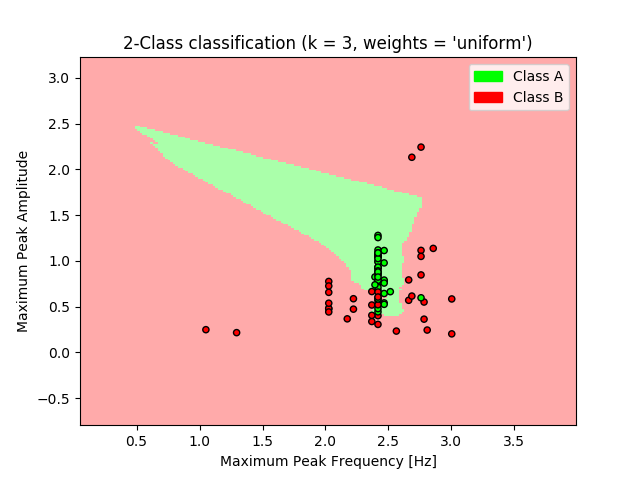
\includegraphics[scale=0.8]{knn_decision_boundary_k_3}
	\decoRule
	\caption{This figure shows the classification boundary for the KNN algorithm with $K=3$ for all of the training data.}
	\label{fig:knn_decision_boundary_k_3}
\end{figure}

A nice way to visualize the results of the classification algorithm with 2-dimensional inputs is to create a decision boundary plot.  A decision boundary is the area in space where the algorithm switches to a different classification.  Figure \ref{fig:knn_decision_boundary_k_3} shows the classification boundary for the KNN algorithm with $K=3$.

Initially, the balanced and imbalanced classes were expected to be easily distinguishable from each other.  Despite not having accurate labels of the experimental data, the imbalanced rotor data was expected to have much higher amplitudes at the rotor frequency; however, from Figure \ref{fig:knn_decision_boundary_k_3}, there isn't a significant difference between the amplitudes of the 2 data classes.

One observation that can be made from the data shown in Figure \ref{fig:knn_decision_boundary_k_3} is that the Class A data seems to have more frequency stability.  The Class A data has a constant frequency of about 2.5 Hz, while the Class B data has varying frequencies.  There is not enough data to make any hard conclusions, but this variance could be caused by either wind speed fluctuations or an actual property of the imbalance.  It is possible that an imbalance in the rotor could cause more variations in rotor speed, despite not having significant amplitude differences.  However, until the data can be accurately labeled, or more experimental data is collected, these classes should remain Class A and Class B to avoid any incorrect assumptions about the rotor imbalance.

\section{Logistic Regression}
\subsection{About the algorithm}
Logistic regression (LR) is a modified version of linear regression that is adapted for classification problems.  Logistic regression minimizes the squared error of a linear combination of the input parameters when passed through a sigmoid function.  To fully understand logistic regression, a brief background of linear regression is required. 

Linear regression is the process of minimizing the least squares cost of a data set with a linear function.  This is a commonly utilized method in curve fitting, but can also be applied to very high order systems.  Mathematically, this means minimizing the cost function shown in Equation \ref{eq:linear_regression_cost_fun}.  The hypothesis is the linear curve fit shown in Equation \ref{eq:linear_regression_hypothesis}.
\begin{align}
	J\left(\vec{\theta}\right) &= \frac{1}{2m} \sum_{i=1}^{m}{\left(h_{\theta}(x_i) - y_i\right)^2} \label{eq:linear_regression_cost_fun} \\
	h_{\theta}(x) &= \mat{x} \cdot \vec{\theta}^T \label{eq:linear_regression_hypothesis} \\
	\vec{\theta} &= [\theta_1, \theta_2, \theta_3, \hdots, \theta_n]
\end{align}

$n$ is the number of parameters (or features) in the input, $\mat{x}$.  $m$ is the number of training examples, which means $\mat{x}$ is of size $[m, n]$ and $\vec{\theta}$ is a vector with $n$ elements.

In order to apply linear regression to classification problems, the sigmoid function is applied to the linear regression hypothesis ($h_{\theta}$).  The sigmoid function is defined in Equation \ref{eq:sigmoid_function} and is visually shown in Figure \ref{fig:sigmoid_plot}.  The sigmoid function is designed to map an input to a value between 0 and 1, which represents the probability that the input is of a certain class.  This sigmoid function is what enables logistic regression to calculate binary outputs.
\begin{equation} \label{eq:sigmoid_function}
	g(z) = \frac{1}{1+e^{-z}}
\end{equation}

\begin{figure}
	\centering
	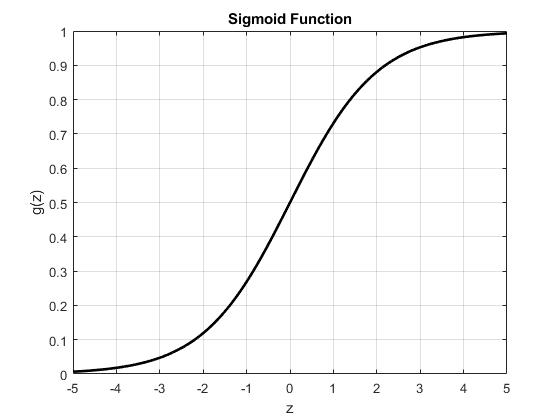
\includegraphics[scale=0.6]{sigmoid_plot}
	\decoRule
	\caption{This figure shows the sigmoid function plot.}
	\label{fig:sigmoid_plot}
\end{figure}

This new hypothesis function (Equation \ref{eq:logistic_regression_hypothesis}) produces a new cost function, shown in Equation \ref{eq:logistic_regression_cost}.
\begin{align}
	J(\theta) &= \frac{1}{m} \sum_{i=1}^{m}{\left[y_i \ln({h_{\theta}(x_i))} + (1-y_i) \ln{(1-h_{\theta}}) \right]}  \label{eq:logistic_regression_cost} \\
	h_{\theta} &= g(\mat{x} \cdot \vec{\theta}^T) = \frac{1}{1+e^{-(\mat{x} \cdot \vec{\theta}^T)}} \label{eq:logistic_regression_hypothesis}
\end{align}

The goal of logistic regression is to create a model that best fits the experimental training data by optimizing the parameters $\vec{\theta}$ to minimize the cost function, $J(\theta)$.  To do this, the gradient descent method is used \cite{gradient_descent}.  To  perform gradient descent, both the cost function and the gradient function of $\vec{\theta}$ are required.  The gradient can be numerically calculated using the finite difference method \cite{finite_difference_method}; however, this is much more computationally intensive than directly calculating the gradient analytically.  The derivative of the sigmoid function is shown in Equation \ref{eq:sigmoid_derivative}.  This produces a simple equation for the gradient of the cost function, which is shown in Equation \ref{eq:logistic_regression_gradient}.
\begin{align}
	g\prime(z) &= g(z) (1-g(z)) \label{eq:sigmoid_derivative} \\
	\frac{\partial J(\theta)}{\partial \theta_j} &= \frac{1}{m} \sum_{i=1}^{m}{\left(h_{\theta}(x_i) - y(i)\right) x_{j,i}} \label{eq:logistic_regression_gradient}
\end{align}

$h_{\theta}$ is defined in Equation \ref{eq:logistic_regression_hypothesis} and $g(z)$ is defined in Equation \ref{eq:logistic_regression_cost}.  In other words, Equation \ref{eq:logistic_regression_gradient} represents an average of $(h-y)x$ for every training example and calculated with respect to each $\theta$ parameter ($j$ is the number of parameters in the model).

\subsection{Training the model}
To train the model, the cost function is minimized using a version of the gradient descent optimization process.  This iterates through various values of $\theta$ that are calculated using the gradient of the cost function.  Figure \ref{fig:logistic_regression_2_feature_cost} shows the cost function over the iteration (training) process.  When the cost function has converged to a minimum, the model training is complete and the model is ready to be validated on the test data.

\begin{figure}
	\centering
	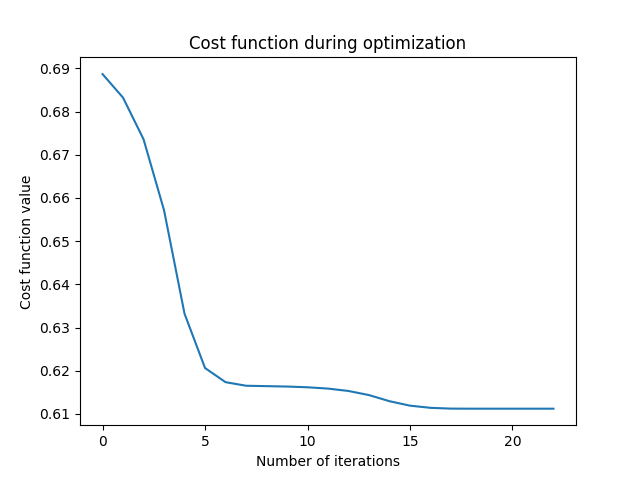
\includegraphics[scale=0.8]{logistic_regression_2_feature_cost}
	\decoRule
	\caption{This figure shows the cost function during the training process.  This model uses 2 features, so the model is trying to optimize $\vec{\theta} = [\theta_1, \theta_2, \theta_3]$ (3 parameters because there is a hidden bias unit).}
	\label{fig:logistic_regression_2_feature_cost}
\end{figure}

\subsection{Applying the model}
Minimizing the cost function results is a trained model that produces the decision boundary shown in Figure \ref{fig:logistic_regression_decision_boundary}.  This model has a pretty poor accuracy of about 67\% on the test data.

\begin{figure}
	\centering
	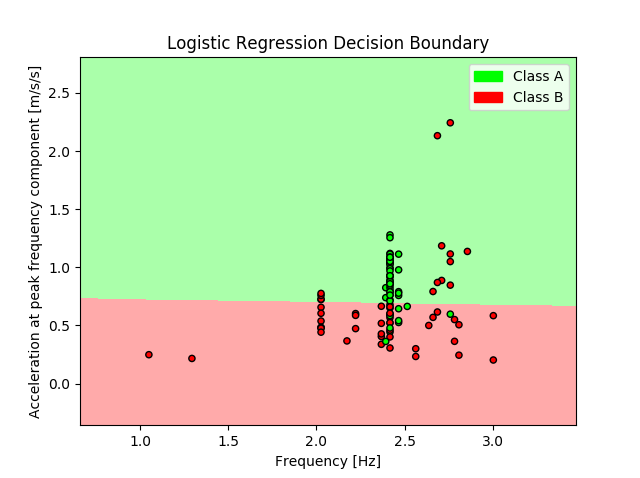
\includegraphics[scale=0.8]{logistic_regression_decision_boundary}
	\decoRule
	\caption{This figure shows the decision boundary from the logistic regression model.  This is a linear model using 2 input parameters and a binary output class.  This model has an accuracy of about 67\% when using the test data set.}
	\label{fig:logistic_regression_decision_boundary}
\end{figure}

To improve this model, the 2 input parameters can be expanded to create a higher order models.  For example, the 2 input features for a linear logistic regression model are shown in Equation \ref{eq:lr_order1}.  To achieve higher order models, the input parameters can be expanded to included the terms for the higher order polynomials.  This will allow the regression to fit parameters to each of the new inputs.  Equation \ref{eq:lr_order2} represents the input variables expanded for a 2nd order model and Equation \ref{eq:lr_order3} represents the input variables expanded for a 3rd order model.  Figure \ref{fig:logistic_regression_order2_decision_boundary} shows the decision boundary for a 2nd order model and Figure \ref{fig:logistic_regression_order3_decision_boundary} shows the decision boundary for a 3rd order model.
\begin{align}
	[x_1, x_2]  \label{eq:lr_order1} \\
	[x_1, x_2, x_1^2, x_1 x_2, x_2^2] \label{eq:lr_order2} \\
	[x_1, x_2, x_1^3, x_1^2 x_2, x_1 x_2^2, x_2^2] \label{eq:lr_order3}
\end{align}

\begin{figure}
	\centering
	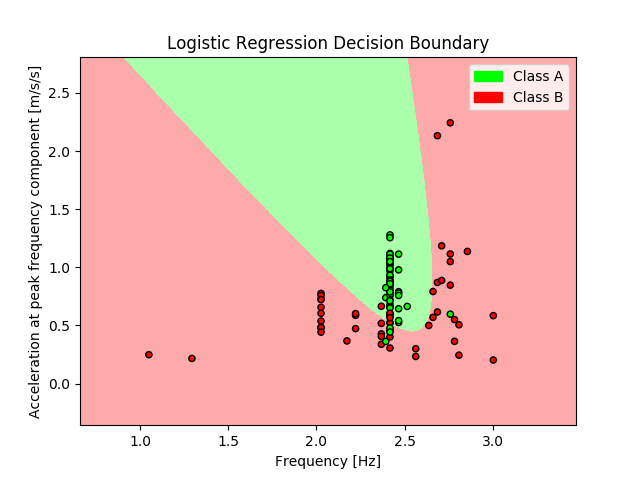
\includegraphics[scale=0.8]{logistic_regression_order2_decision_boundary}
	\decoRule
	\caption{This figure shows the decision boundary from the logistic regression model.  This is a 2nd order model using 2 input parameters and a binary output class.  This model has an accuracy of about 85\% when using the test data set.}
	\label{fig:logistic_regression_order2_decision_boundary}
\end{figure}

\begin{figure}
	\centering
	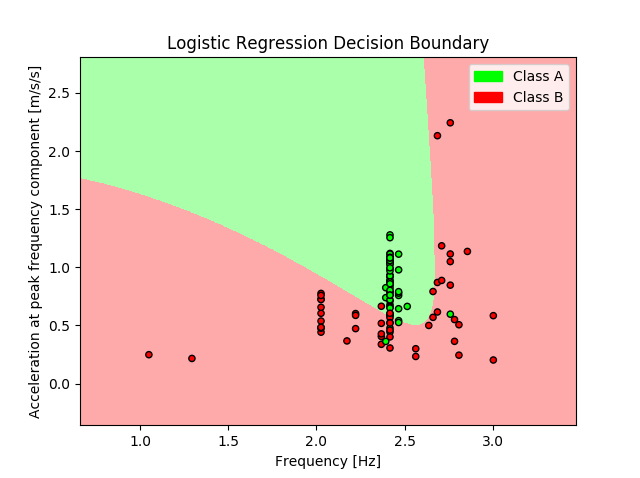
\includegraphics[scale=0.8]{logistic_regression_order3_decision_boundary}
	\decoRule
	\caption{This figure shows the decision boundary from the logistic regression model.  This is a 3rd order model using 2 input parameters and a binary output class.  This model has an accuracy of about 85\% when using the test data set.}
	\label{fig:logistic_regression_order3_decision_boundary}
\end{figure}

In fact, the order can keep getting increased until the model fits the training data perfectly.  This is called over-fitting and is a problem with higher order machine learning models.  Figure \ref{fig:logistic_regression_order10_decision_boundary} shows an example of a 10th order model that has some over-fitting problems.  It is unlikely that the small region separating the Class A sections (at about 2.5 Hz and 1.5 m/s/s) belongs to Class B.  In order to solve the problem of over-fitting, a regularization term can be added to the cost function equation.  This regularization term, $\lambda$, effectively reduces the impact that the optimization parameters have on the cost calculation, which keeps the optimized parameters small.  This reduces the ``strength" of the regression model and can help eliminate over-fitting problems.  Equation \ref{eq:logistic_regression_cost_reg} shows the new logistic regression cost function with a regularization term applied.  The new gradient function can be derived with the regularization term, as shown in Equation \ref{eq:logistic_regression_gradient_reg}.

\begin{figure}
	\centering
	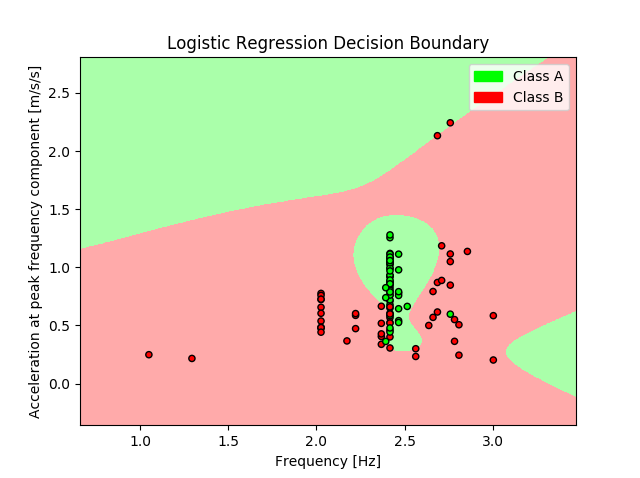
\includegraphics[scale=0.8]{logistic_regression_order10_decision_boundary}
	\decoRule
	\caption{This figure shows the decision boundary from the logistic regression model.  This is a 10th order model using 2 input parameters and a binary output class, and has an over-fitting problem.  This model has an accuracy of about 81\% when using the test data set.  Notice that the accuracy of the over-fitting model on the test data is lower than the lower order models shown in Figure \ref{fig:logistic_regression_order2_decision_boundary}.}
	\label{fig:logistic_regression_order10_decision_boundary}
\end{figure}

\begin{align}
	J(\theta) &= \frac{1}{m} \sum_{i=1}^{m}{\left[y_i \ln({h_{\theta}(x_i))} + (1-y_i) \ln{(1-h_{\theta}}) \right]} + \frac{\lambda}{2m} \sum_{j=1}^{n}{\theta_j^2} \label{eq:logistic_regression_cost_reg} \\	
	\frac{\partial J(\theta)}{\partial \theta_j} &= \frac{1}{m} \sum_{i=1}^{m}{\left(h_{\theta}(x_i) - y(i)\right) x_{j,i}} + \frac{\lambda}{m} \theta_j\label{eq:logistic_regression_gradient_reg}
\end{align}

Adding regularization to the 10th order model shown in Figure \ref{fig:logistic_regression_order10_decision_boundary}, can result in a much better fitting model for the data.  Figure \ref{fig:logistic_regression_order10_decision_boundary_reg} shows the result of a regularization term of $\lambda=3$.

\begin{figure}
	\centering
	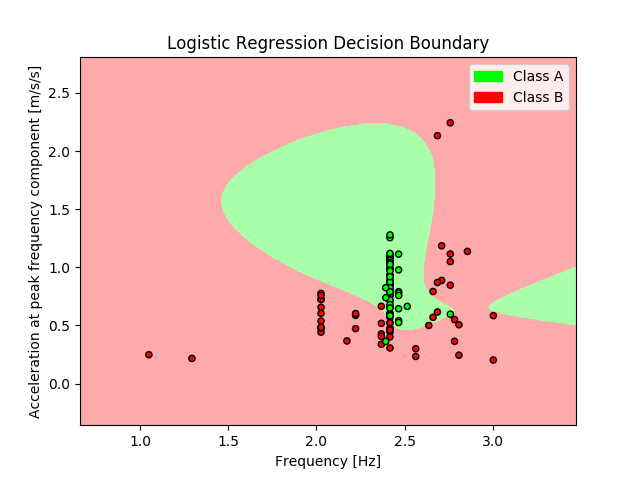
\includegraphics[scale=0.8]{logistic_regression_order10_decision_boundary_reg}
	\decoRule
	\caption{This figure shows the decision boundary from the logistic regression model using a regularization term of $\lambda=3$.  This is a 10th order model using 2 input parameters and a binary output class.  This model has an accuracy of about 86\% when using the test data set, which is higher than the 10th order model with no regularization (Figure \ref{fig:logistic_regression_order10_decision_boundary}).}
	\label{fig:logistic_regression_order10_decision_boundary_reg}
\end{figure}

The logistic regression function outputs the probability that the data set falls into a certain class.  This means that for most decision boundary plots, the data set is classified as Class A if the probability is greater than 50\% and the data is classified as Class B if the probability is less than 50\%.  The decision boundary can also include the probability to produce a smooth gradient plot as in Figure \ref{fig:logistic_regression_decision_boundary_smooth}.

\begin{figure}
	\centering
	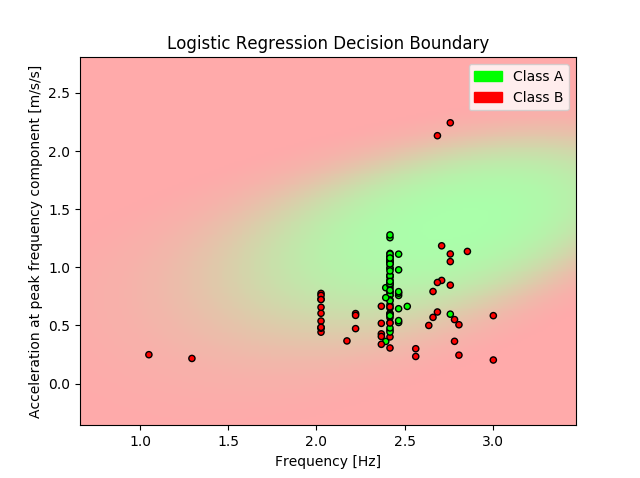
\includegraphics[scale=0.8]{logistic_regression_decision_boundary_smooth}
	\decoRule
	\caption{This figure shows the probability of the model classifying certain data sets as Class A and Class B.  This model was trained with an order of 3 and a regularization parameter of $\lambda=1$.  The background color of the plot represents the probability of the data set being classified as Class A, with solid green being about 99\% certainty and solid red being about 1\% certainty.}
	\label{fig:logistic_regression_decision_boundary_smooth}
\end{figure}



\subsection{Using a complete feature set}
The logistic regression models in the previous section use only 2 features from the entire data set (the features shown in Figure \ref{fig:max_balanced_freq_mag}).  This is convenient because it is easy to conceptualize and visualize.  The decision boundaries for models with 2 features can be analyzed using plots like Figure \ref{fig:logistic_regression_order10_decision_boundary_reg}.  A better version of the model would use all of the frequency spectrum data as inputs to the model.  This means that instead of using the peak amplitude and corresponding maximum frequency as model inputs, the entire FFT could be used.

Using the whole frequency spectrum means the model will have 256 features (one for the magnitude of each frequency component).  This is a lot of features to use for the KNN algorithm and will be far too slow when more training data is acquired.  The benefit of regression-based models is that the computational cost to predict the class of new data remains the same regardless of how many training examples are used to optimize the model parameters.  This means that using more data will just improve the model without slowing down the real-time calculations (it will, however, make the training time much slower).

Figure \ref{fig:logistic_regression_all_features_cost} shows a plot of the cost function value during the training process.  This is a common way of visually ensuring the model has converged to a local minimum. This produces an accuracy score of 95\% on the training data which is much higher than the scores from the 2-feature models in the previous section.

\begin{figure}
	\centering
	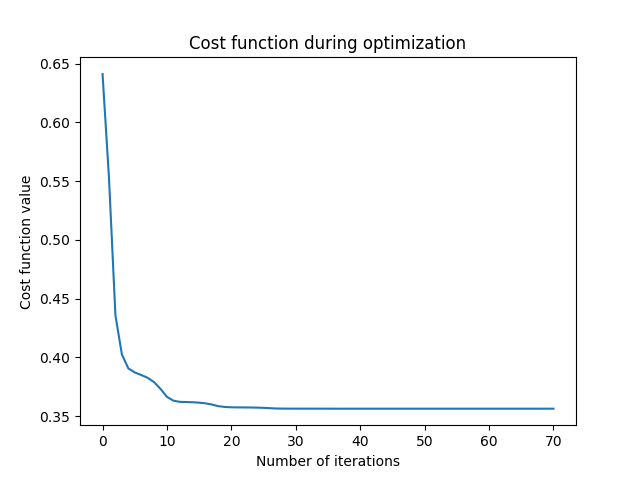
\includegraphics[scale=0.8]{logistic_regression_all_features_cost}
	\decoRule
	\caption{This figure shows the cost function value during the training process with a regularization term of $\lambda=1$.  In this model, all 256 features are used as inputs.}
	\label{fig:logistic_regression_all_features_cost}
\end{figure}

To better understand the results of the training process, the model parameters are plotted in Figure \ref{fig:logistic_regression_model_parameters}.  This shows each of the parameters in $\vec{\theta}$ and the corresponding frequencies they are correlated to.  To calculate the probability of the turbine being in a specific class, these parameters are multiplied with the FFT results and passed through the sigmoid function, as shown in Equation \ref{eq:logistic_regression_hypothesis}.

From inspecting Figure \ref{fig:logistic_regression_model_parameters}, it appears as though the frequency around 2.5 Hz is weighted the most, with some of the surrounding frequencies having small negative weights.  The logistic regression model essentially ``learns" that it should inspect the rotor frequency to classify the state of the turbine.    It is also interesting that frequencies +/- 0.5 Hz from the strongest component in $\vec{\theta}$ have the biggest negative weights.  From a visual inspection of the training data in one of the previous decision boundary plots (like Figure \ref{fig:logistic_regression_order10_decision_boundary_reg}), it appears as though data is likely to belong to Class A if the frequency is fairly constant around 2.5 Hz.  If the frequency diverges from this value, the training data generally falls into Class B, which is how the logistic regression model is analyzing the data and predicting the turbine state.

\begin{figure}
	\centering
	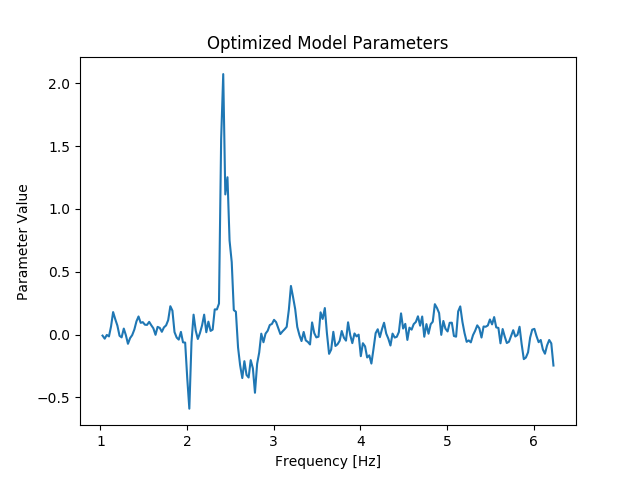
\includegraphics[scale=0.8]{logistic_regression_model_parameters}
	\decoRule
	\caption{This figure shows the optimized model parameters for the logistic regression model using all the input features.  Each parameter corresponds to a specific frequency, which means that this function gets multiplied by the FFT of each data set and used to calculate the probability that the turbine is either balanced on not balanced.}
	\label{fig:logistic_regression_model_parameters}
\end{figure}

\section{Neural Network}

\subsection{About the algorithm}
A neural network is an algorithm that resembles the neurons in the brain.  This is essentially a more complicated version of logistic regression, and is capable of training nonlinear models.  In some of the previous models (Such as the models in Figure \ref{fig:knn_decision_boundary_k_3} and Figure \ref{fig:logistic_regression_decision_boundary}), the DFT data was condensed down into 2 variables, which are the magnitude of the maximum frequency component and its corresponding frequency.  These variables were selected from intuition about the tower dynamics; however, there may be 2 different abstract features that better describe the system.  In order to find the 2 best features that describe the system, a neural network can be set up as shown in Figure \ref{fig:neural_network_diagram}.  This network has 3 layers, which include the input layer, hidden layer, and output layer.  The hidden layer contains 2 units, which are abstract features that can be fit to a linear model.  These 2 features should be a better indicator of the state of the turbine than the frequency and magnitude values previously used.  The (+1) units in the network represent bias units that are injected into the network to apply a constant bias to each set of parameters or features.

\begin{figure}
\centering
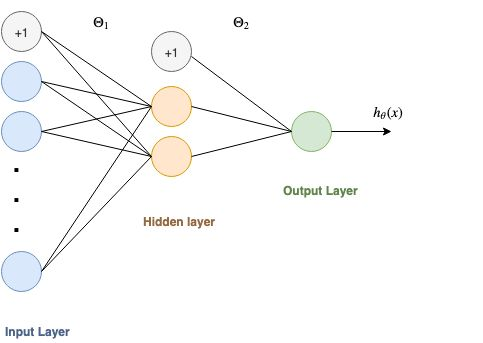
\includegraphics[scale=0.8]{neural_network_diagram}
\decoRule
\caption{This figure shows a neural network diagram for the turbine model.  The input layer contains the 256 DFT values, and the output layer contains the predicted probability that the turbine is balanced or not balanced.  The hidden layer represents some abstract features that can be used to predict the state of the turbine with a linear model.  This figure was created with Draw.io.}
\label{fig:neural_network_diagram}
\end{figure}

For each layer, the value of each unit can be calculated by multiplying the weight matrix by the previous layer units and applying the sigmoid function, $g(z)$ (Equation \ref{eq:sigmoid_function}).  For example, the values in layer 2 ($\mat{a_2}$) can be calculated using Equation \ref{eq:nn_layer_2}.
\begin{equation} \label{eq:nn_layer_2}
	\mat{a_2} = g\left(\mat{X} \cdot \mat{\Theta_1}\right)
\end{equation}

In Equation \ref{eq:nn_layer_2}, $\mat{X}$ is the input data of size $[m,n]$, where $m$ is the number of training examples, and $n$ is the number of features (256 if all the DFT values are used).  $\mat{\Theta_1}$ is the matrix of weight values that is optimized during the training process.

The hypothesis of the model in Figure \ref{fig:neural_network_diagram} is calculated using Equation \ref{eq:nn_hypothesis}.  This is the predicted probability that the turbine is balanced or unbalanced for all the training examples.
\begin{equation} \label{eq:nn_hypothesis}
	\vec{h}_{\theta} = g\left(\mat{a2} \cdot \mat{\Theta_2} \right)
\end{equation}

The squared difference cost function of the neural network diagram is shown in Equation \ref{eq:nn_cost_function}.
\begin{equation} \label{eq:nn_cost_function}
	J(\theta) = \frac{1}{m} \sum_{i=1}^{m}{\sum_{k=1}^{K}{\left[-y_{k,i} \ln{(h_{\theta}(x_i)} - (1-y_{k,i}) \ln{(1-h_{\theta}(x_i))} \right]}}
\end{equation}

To calculate the analytic gradient of the cost function back propagation is required.  Back propagation is an algorithm is derived from calculus to determine the gradient of a neural network.  As the name suggests, this method starts from the neural network output and calculates the error of each layer, which can be related to the gradient.  First, $\delta$ for each layer is calculated as shown in Equation \ref{eq:backprop_delta_3} and Equation \ref{eq:backprop_delta_2}.  $\odot$ is the element-wise operator, which can also be represented as $\code{.*}$ in MATLAB.  It is also important to remove the term for $\delta_{2,0}$ because there is no gradient term defined for the bias unit in the second layer.
\begin{align}
	\vec{\delta}_3 &= \vec{h} - y \label{eq:backprop_delta_3}\\
	\vec{\delta}_2 &= \mat{\Theta_2}^T \cdot \vec{\delta}_3 \odot g\left(\mat{X} \mat{\Theta_1}\right) \label{eq:backprop_delta_2}
\end{align}

Using $\delta$, the gradient of $\mat{\Theta_1}$ and $\mat{\Theta_2}$ can be calculated using Equation \ref{eq:backprop_theta1_grad} and Equation \ref{eq:backprop_theta2_grad}.
\begin{align}
	\frac{\partial J(\Theta)}{\partial \Theta_1} &= \frac{1}{m} \left(\vec{\delta}_2^T \cdot \vec{a}_1 \right) \label{eq:backprop_theta1_grad} \\
	\frac{\partial J(\Theta)}{\partial \Theta_2} &= \frac{1}{m} \left(\vec{\delta}_3^T \cdot \vec{a}_2 \right) \label{eq:backprop_theta2_grad}
\end{align}

The back propagation method for calculating the gradient is much faster than using a numerical method such as the finite difference approximation.  Many optimization algorithms will default to the forward finite difference gradient approximation if a gradient function is not supplied, so it is important to provide the optimization function with both the cost function and gradient function.

\subsection{Training the model}
Now that a neural network model has been set up and mathematically described, the model needs to be trained.  In other words, this means finding values for $\mat{\Theta_1}$ and $\mat{\Theta_2}$ that minimize the cost function, $J(\Theta)$.  Optimization functions generally assume the parameters are in a single vector (rather than 2 separate matrices).  $\mat{\Theta_1}$ and $\mat{\Theta_2}$ can be flattened into a single vector, and unrolled into matrices when they are used in calculations.  An example of flattening the parameters into a single vector using Python (with the numpy package) is shown below:
\begin{equation} \nonumber
	\code{nn\_params = numpy.append(Theta1.flatten(), Theta2.flatten())}
\end{equation}

To train the model, the parameters are minimized using the $\code{fmincg}$ function from the $\code{scipy.optimize}$ package.  This is a nonlinear conjugate gradient algorithm that was developed by Polak and Ribliere \cite{numerical_fmin_cg}.  Figure \ref{fig:nn_cost_function} shows the cost function during the optimization process.  \textit{It is very important that the parameters $\mat{\Theta_1}$ and $\mat{\Theta_2}$ are initialized randomly before the training process.}  If all of the values are initialized to zero, the model will not develop distinct weights for each connection.  This is a property of neural networks and is usually standard practice when training models.

\begin{figure}
\centering
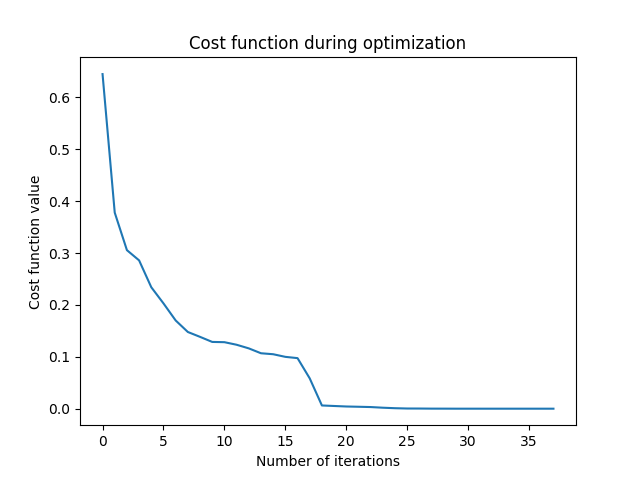
\includegraphics[scale=0.8]{nn_cost_function}
\decoRule
\caption{This figure shows the cost function of the neural network in Figure \ref{fig:neural_network_diagram} during the optimization process. This figure was created with Python.}
\label{fig:nn_cost_function}
\end{figure}

\subsection{Applying the model}
Minimizing the cost function results in optimized parameters for $\mat{\Theta_1}$ and $\mat{\Theta_2}$.  Figure \ref{fig:nn_hidden_layer_decision_boundary} shows a decision boundary plot using the hidden layer activations as input variables.  When this plot is compared to the 2-variable data in Figure \ref{fig:logistic_regression_order10_decision_boundary_reg}, the variables in Figure \ref{fig:nn_hidden_layer_decision_boundary} seem to be a much better choice of inputs.  These are abstract variables that can be fit to a linear model (notice the straight line defining the decision boundary) to describe the state of the turbine.

For clarification, the data shown in Figure \ref{fig:nn_hidden_layer_decision_boundary} are internal variables used in the neural network classification algorithm and are created from the same 256-point DFT data as the previous plots.  This model has a prediction accuracy of 85 - 95\% on the test data depending on how the variables are randomly initialized.  This variability is a result of a lack of training and test data.  For a proper neural network model more data is always better.  Unlike the nonlinear KNN algorithm, neural networks are nonlinear algorithms that have a relatively constant prediction time.  More data will not change the computational time required to calculate an output with a new test data set.

\begin{figure}
\centering
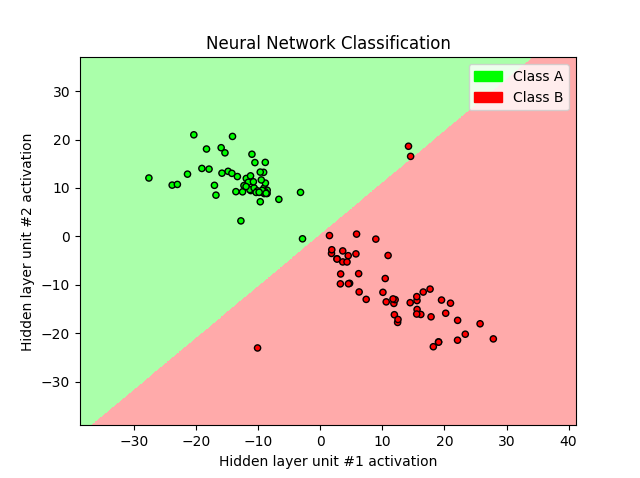
\includegraphics[scale=0.8]{nn_hidden_layer_decision_boundary}
\decoRule
\caption{This figure shows the decision boundary of the hidden layer activations of the neural network model shown in Figure \ref{fig:neural_network_diagram}.  These 2 parameters are the abstract variables that the network created to linearly classify the system. This figure was created with Python.}
\label{fig:nn_hidden_layer_decision_boundary}
\end{figure}

\subsubsection{Increasing the architecture complexity}
\todo{complete or delete this section}
The previous model was designed using the structure in Figure \ref{fig:neural_network_diagram}, which was chosen because the hidden layer only has 2 units.  This makes it easy to visualize the intermediate results of the model.  More complicated neural network models are possible, but they are harder to conceptualize and visualize.  For example, Figure \ref{fig:neural_network_diagram_complex} shows a version of a 3 

\begin{figure}
\centering
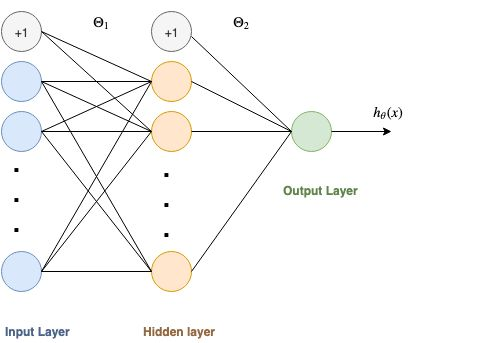
\includegraphics[scale=0.8]{neural_network_diagram_complex}
\decoRule
\caption{This figure shows the decision boundary of the hidden layer activations of the neural network model shown in Figure \ref{fig:neural_network_diagram}.  These 2 parameters are the abstract variables that the network created to linearly classify the system. This figure was created with Python.}
\label{fig:neural_network_diagram_complex}
\end{figure}


\todo{Add next steps and fix bibliography}

